\subsection{Interactive Debugging and Chat Interface}
\label{sec:method_interactive}

\subsubsection{Live Chat Interface}

\textcolor{blue}{Batch evaluation is necessary for aggregate comparison, but it is insufficient for rapid iteration on agent design. EABench therefore ships an interactive Streamlit application (Figure~\ref{fig:debug_interface}) in which the same runtime used for evaluation can be exercised through a live chat interface. A researcher selects an agent configuration, a tenant dataset, and a user persona from the sidebar, then issues free-form queries to inspect the agent's behavior under that persona's access scope. The main panel displays the agent's structured response with inline citation markers and a references section listing source artifacts with metadata (type, author, date, entity ID). This mode is especially valuable during prompt engineering and tool-ablation studies, because it shortens the loop between a configuration change and a concrete behavioral observation.}

\subsubsection{Debugging Facilities}

\textcolor{blue}{The interactive layer exposes the pieces of evidence that matter for debugging enterprise agents. The sidebar navigation provides four views: \emph{Chat} for live query exploration, \emph{Evaluation} for batch result inspection, \emph{Side-by-Side Comparison} for contrasting agent configurations on the same query, and \emph{Data Generator} for creating new tenant datasets. In the Chat view, the agent's response includes inline citation markers that link to a References section with full artifact metadata---type, author, date, and entity ID---enabling a researcher to verify each cited source against the tenant corpus. The Login panel displays the active user's role and ID, making access-scope constraints transparent. These views make it possible to distinguish several common failure modes: the agent may choose the wrong tool, retrieve weak evidence, lose track of a multi-hop chain, or cite the right artifact incorrectly. Because these signals are surfaced directly, EABench supports debugging by diagnosis rather than by prompt trial-and-error alone.}

\begin{table}[t]
\centering
\caption{\textcolor{blue}{Debugging surfaces exposed by the interactive workflow.}}
\label{tab:debug_surfaces}
\small
{\color{blue}
\begin{tabular}{p{0.28\linewidth}p{0.60\linewidth}}
\toprule
\textbf{Surface} & \textbf{What it reveals} \\
\midrule
Agent \& tenant selectors & Switch agent configuration and corpus without restarting \\
User persona login        & Role, user ID, and access scope active for the current session \\
Inline citations          & Numbered markers in the response linking to specific source artifacts \\
References panel          & Full metadata (type, author, date, entity ID) for each cited artifact \\
Side-by-side comparison   & Contrast two agent configurations on the same query and persona \\
Batch evaluation view     & Aggregate metrics and per-case drill-down for completed eval runs \\
\bottomrule
\end{tabular}
}
\end{table}

\begin{figure}[t]
\centering
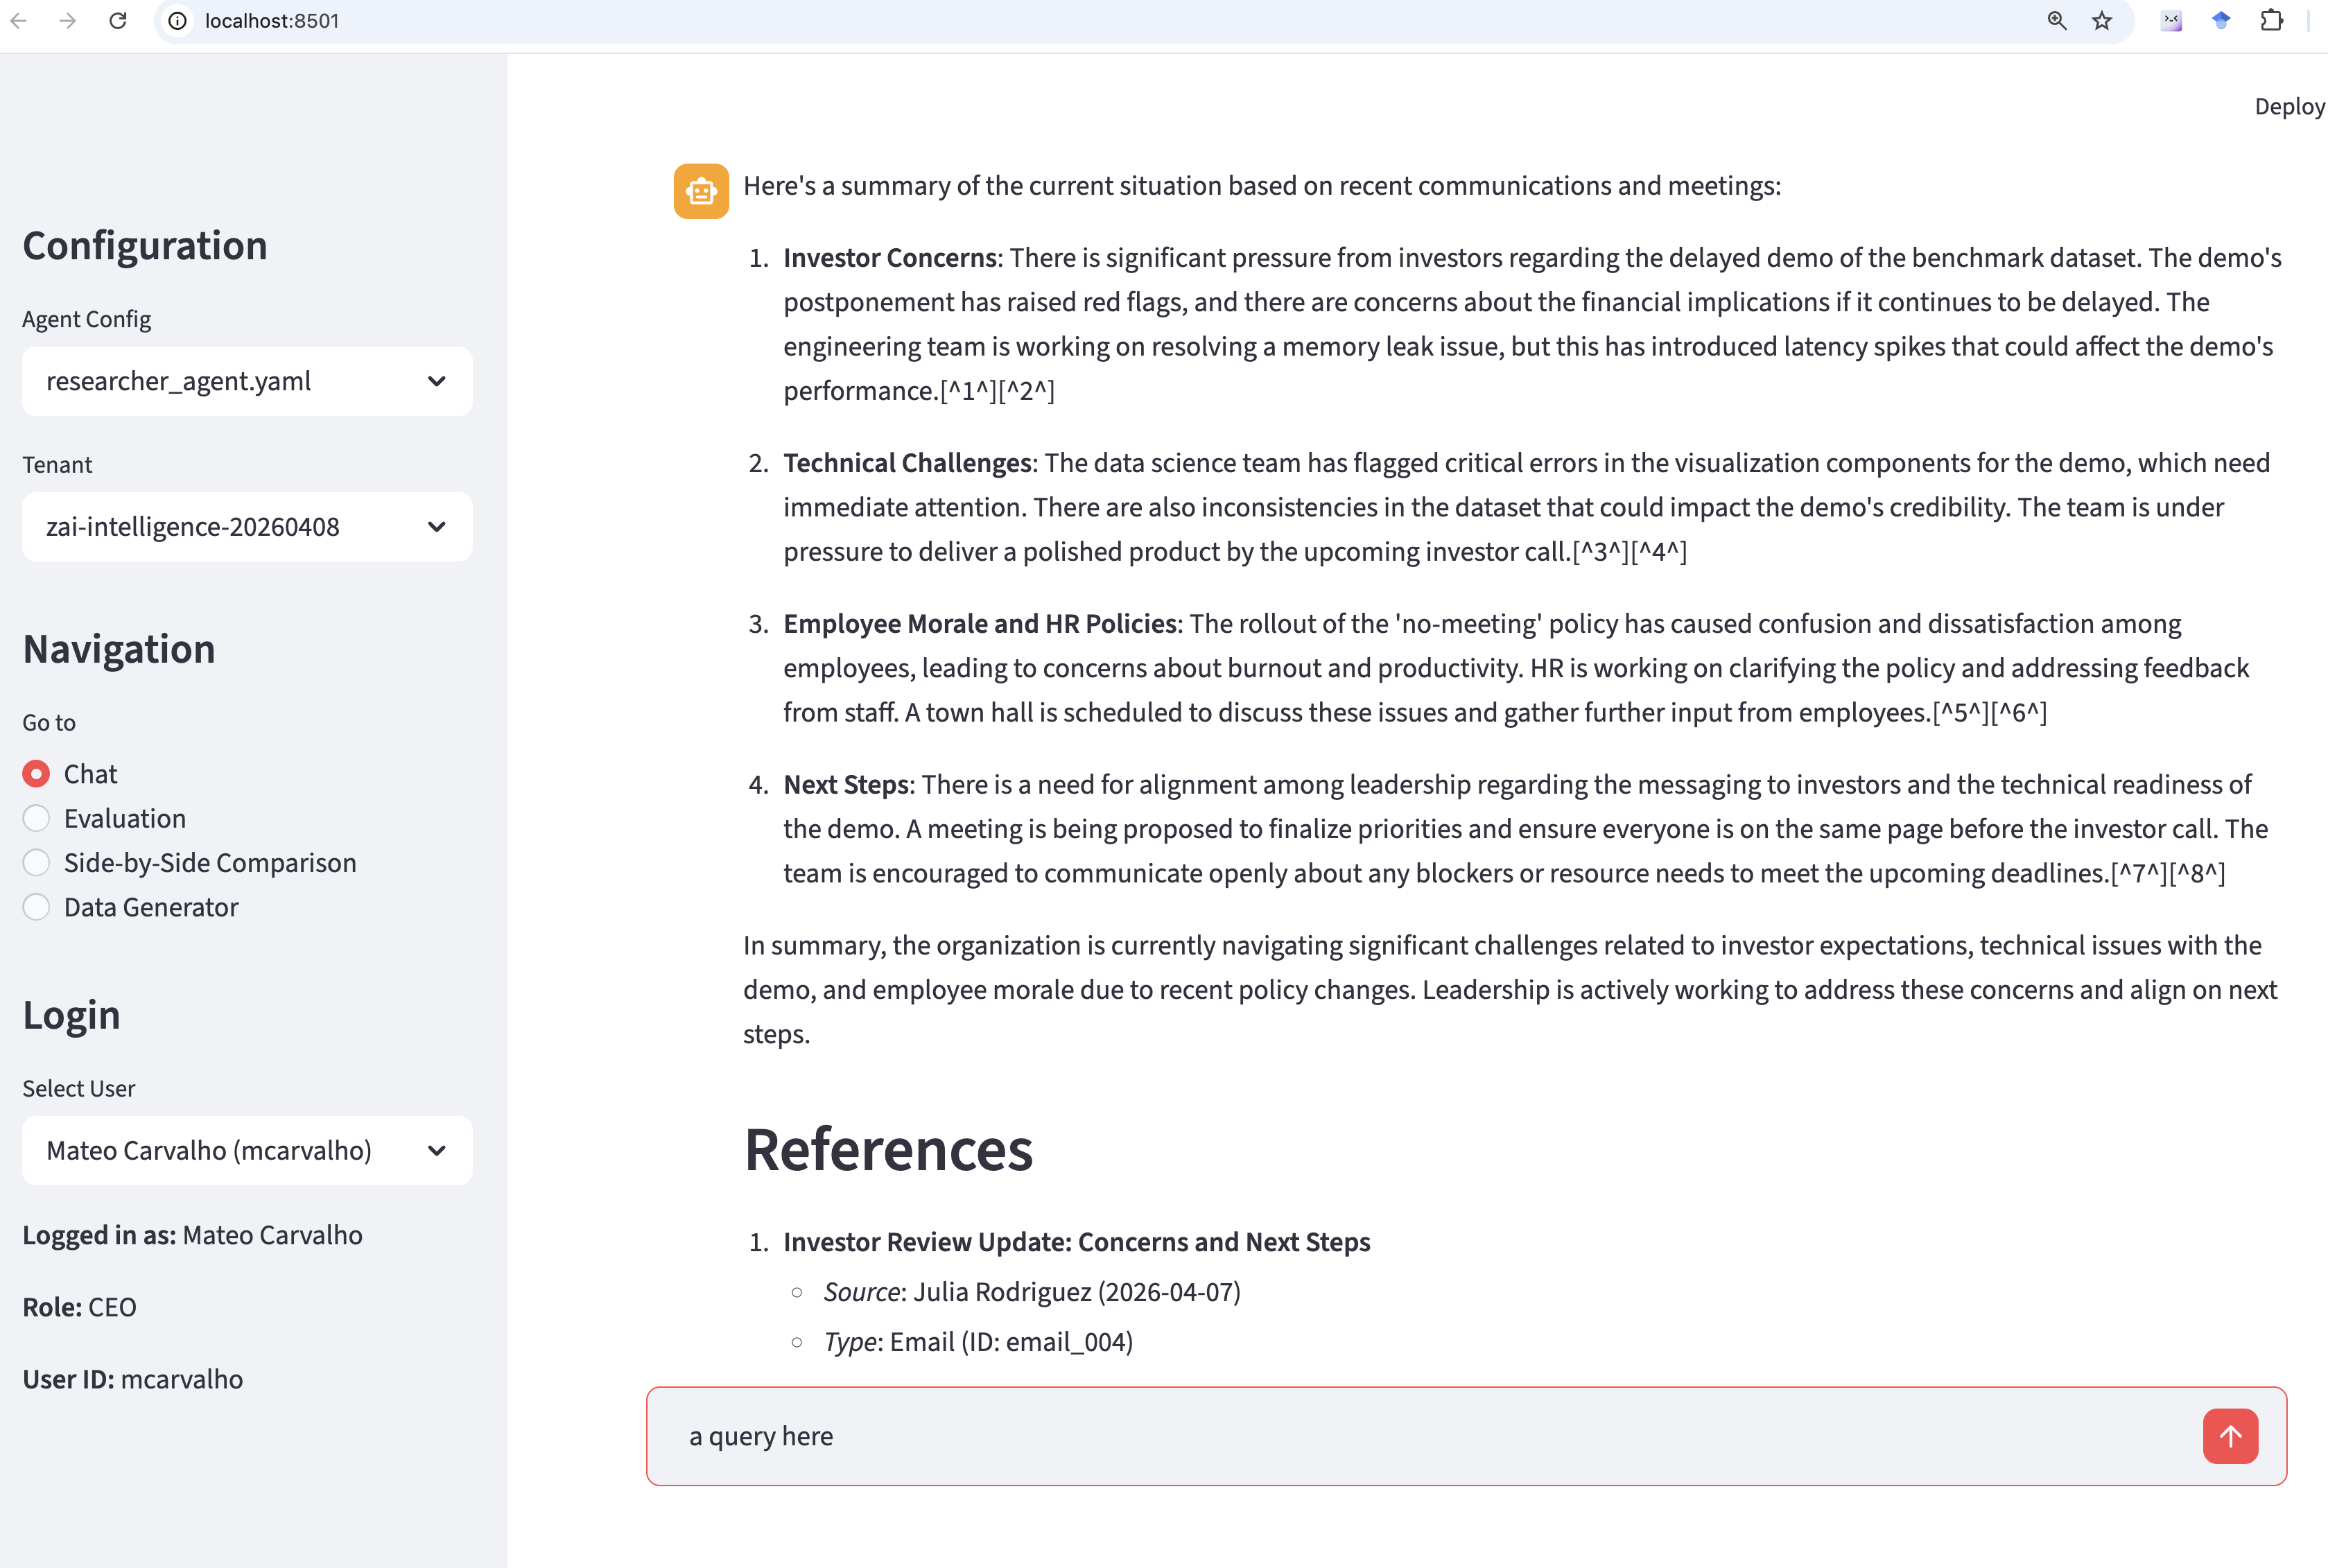
\includegraphics[width=\linewidth]{figures/eabench_screenshot.png}
\caption{\textcolor{blue}{EABench interactive chat interface. The left sidebar provides configuration controls (agent strategy, tenant, and user persona); the main panel displays the agent's structured response with inline citation markers and a references section listing source artifacts with metadata. A query input box at the bottom enables iterative exploration under the selected persona.}}
\label{fig:debug_interface}
\end{figure}

\subsubsection{User Experience Testing}

\textcolor{blue}{The interactive workflow is also useful for evaluating enterprise usability beyond aggregate benchmark scores. Researchers can replay the same case under multiple personas, inspect which artifacts become visible or hidden, and compare how different runtime configurations explain uncertainty to the user. In this sense, the interactive interface serves as a bridge between formal benchmarking and deployment-oriented validation: it preserves reproducibility while surfacing the qualitative details that determine whether an enterprise agent is trustworthy in practice.}